\chapter{Linear elasticity equation -- Loaded elastic beam -- 3D}

\modinfo{Directory}{ElasticBeam3D}
\modinfo{Solvers}{\Idx{StressSolve}}
\modinfo{Tools}{\Idx{ElmerGUI}}
\modinfo{Dimensions}{3D, Steady-state}
\modinfo{Author}{Peter R{\aa}back}


\subsection*{Case definition}

Assume a homogenous, elastic beam being rigidly supported on one 
end. On the other end it is subjected with a load of 2000~N
resulting from an attached object in the gravitational field. The gravity affects also the beam itself.
The length of the beam is 1~m and the thickness is 0.05~m, and the width 
0.1~m.
Material properties of the beam are those of dry pine timber:
Poisson 
ratio 0.37, Young's modulus $10\cdot 10^9$N/m$^2$, and density 550~kg/m$^3$. 
The problem is to solve the displacement and stress field of the beam.  
Here the \texttt{StressSolve} routine based on the 
linear theory of elasticity is applied.


\subsection*{Solution procedure}

The mesh is given in ElmerGrid format in file \texttt{beam3d.grd}, load this file.
\ttbegin
File 
  Open -> beam3d.grd
\ttend
You should obtain your mesh and may check that it consists of 6073 nodes and of 
1200 quadratic hexahedral elements. The second order elements give
improved accuracy compared to the first order elements as they avoid the phenomenom known as locking.
\begin{figure}[h!]
\begin{center}
  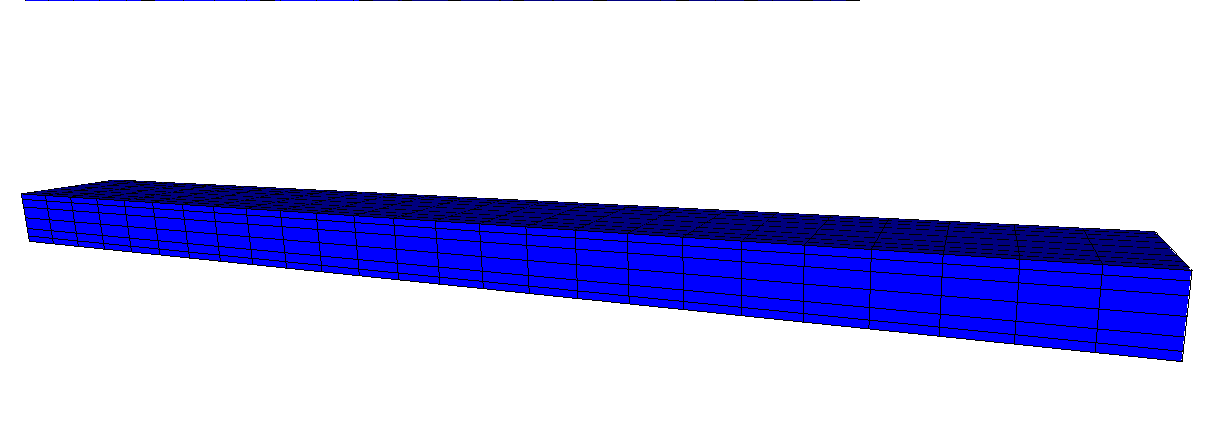
\includegraphics[width=0.8\textwidth,viewport=0 0 1230 300,clip]{beam_mesh}
  \caption{The mesh used in the computations}
  \label{fig:elast_mesh}
\end{center}
\end{figure}

After we have the mesh we start to go through the Model menu from the top to bottom. 
In the Setup we choose things related to the whole simulation such as file names, 
time stepping, constants etc.
The simulation is carried in steady-state in 3-dimensional Cartesian
coordinates. 
\ttbegin
Model
  Setup 
    Simulation Type = Steady state
    Steady state max. iter = 1
\ttend

In the Equation section we choose the relevant equations which in this case only includes 
the \texttt{Linear elasticity} equation
which solves the problem according to 
linear elastic theory. We also want to compute the stresses as a post-processing step.
For the linear system solvers we change the default settings in order
to obtain a better convergence in this case. As the equation is fully linear
we also eliminate the non-linear iteration loop. 
\ttbegin
Model
  Equation
    Name = Elasticity
    Apply to Bodies = Body 1
    Linear elasticity
      Active = on
      Calculate Stresses = on
    Edit Solver Setting
      Linear System
        Method = Iterative / GCR
        Preconditioning = ILU1
      Nonlinear system 
        Max. iterations = 1
      Apply
    Add 
    OK
\ttend        

The Material section includes all the material parameters.
They are divided into generic parameters which are direct properties of the material
without making any assumptions on the physical model, such as the mass. Other properties assume
a physical law, such as Young's modulus and Poisson ratio. 
\ttbegin
Model
  Material
    Name = Pine
    General 
      Density = 550 
    Linear Elasticity 
      Youngs Modulus = 10.0e9
      Poisson ratio = 0.37
    Apply to Bodies = Body 1 
    Add
    OK
\ttend

In this case there is a body force i.e. the gravity acting on the beam.
We assume that the gravity points to the negative $y$ direction.
\ttbegin
Model
  BodyForce
    Name = Gravity
    Linear Elasticity 
      Force 2 = $ -9.81 * 550
    Apply to Bodies = Body 1 
    Add
    OK
\ttend
Here we use a \texttt{MATC} expression for computing the volume force. This
expression is constant and is computed when the command file is interpreted.

Convergence should be obtained with the default 
initial condition i.e. zero for all fields, hence no initial condition is applied.

The first boundary condition fixes the beam rigidly at the wall.
The second boundary condition distributes the load of 2000~N uniformly on the 
area of 5.0e-3~m$^2$.
\ttbegin
Model
  BoundaryCondition
    Name = Wall
    Linear elasticity
      Displacement 1 = 0.0
      Displacement 2 = 0.0
      Displacement 3 = 0.0
    Add
    New

    Name = Mass
    Linear elasticity 
      Force 2 = -4.0e5
    Add 
\ttend   

The conditions may also be assigned to boundaries in the Boundary condition menu, or 
by clicking with the mouse. Here we use the latter approach as that spares us of the 
need to know the indexes of each boundary. 
\ttbegin
Model
  Set boundary properties
    Choose the wall end of the beam -> set boundary condition Wall
    Choose the other end of the beam -> set boundary condition Mass
\ttend

For the execution 
ElmerSolver needs the mesh files and the command file. We have now basically defined
all the information for ElmerGUI to write the command file. After writing it we may also visually 
inspect the command file.
\ttbegin
Sif 
  Generate
  Edit -> look how your command file came out  
\ttend

Before we can execute the solver we should save the files in a directory. The project includes
all the files needed to restart the case.
\ttbegin
File 
  Save Project
\ttend

After we have successfully saved the files we may start the solver
\ttbegin
Run
  Start solver
\ttend
The simulation may take a minute or so depending on the 
speed of the processor.
This time the convergence monitor does not have a meaningful output since 
of the different steps only one is related to the actual solution and the six other
ones to the computation of stresses with the Galerkin method.


\subsection*{Results}

When there are some results to view we may start the postprocessor, this time we use Paraview.
\ttbegin
Run
  Start Paraview
\ttend
Choose the \texttt{displacement} as the color field to plot.
The maximum displacement is $6.36$~cm 
You may also choose various stress components, or the von Mises stress.
Also you may choose to see \texttt{Surface With Edges} to visualize the mesh also. 
The resulting picture is shown in Fig~\ref{fig:beam_stresses}
\begin{figure}[h!]
\begin{center}
  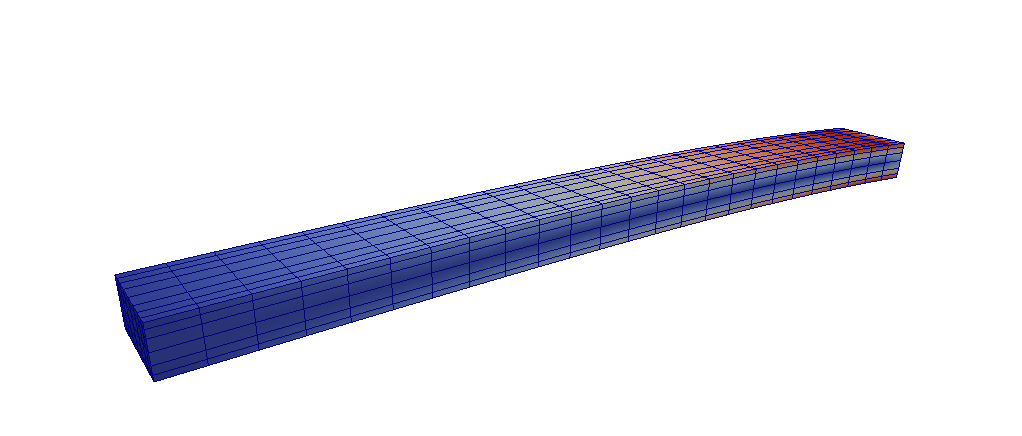
\includegraphics[width=0.8\textwidth]{beam_vonMises}
  \caption{The displaced shape of the elastic beam colored with the 
  von Mises stresses.}
  \label{fig:beam_stresses}
\end{center}
\end{figure}

Note that the displacements are so large that the assumption of linearity may be severely questioned.
When further increasing the loading one should resort to a solver that is able to catch the 
geometric non-linearities -- the ElasticSolver.


\subsection*{Extra task: Gravity in $x$ direction}

The beam should be more rigid if the beam is oriented differently.
For that aim, change the direction of gravity to orient in the negative $x$.
Change the body force
\ttbegin
Model
  BodyForce
    Linear Elasticity 
      Force 1 = $ -9.81*550
    Update
    OK
\ttend
and the boundary condition
\ttbegin
Model
  BoundaryCondition
    Linear elasticity 
      Force 1 = -4.0e5
    Update
    OK
\ttend   
The rigidity should scale as $dh^3$ and hence the maximum displacement should be reduced roughly 
to one quarter of the original.
 

\vfill
\mbox{}
